\documentclass[letterpaper,12pt]{article}

% Packages
\usepackage{enumitem}  % For customized lists
\usepackage{hyperref}  % For hyperlinks
\usepackage{geometry}  % For setting page margins
\usepackage{titling}   % For customizing the title
\usepackage{amsmath}   % For math symbols and equations
\usepackage{graphicx}
\graphicspath{ {./} }
% Set page margins
\geometry{margin=1in}

\begin{document}

\title{Radon Emanation Analysis Notes: Run 733}
\author{H. Ryott Glayzer\ Lab Assistant\ SD Mines}
\date{\today}

\maketitle

\section*{First Analysis}

\textbf{Plots will be stored at \$RNDATA/Run\_733/B}

\paragraph{Visual Inspection of Raw Data}
Upon first inspection, a pattern of periodic gain shifts is apparent in the data.
Appeas to have \~24h period.
It is obvious where the files were overwritten due to run 734.

\paragraph{Hours Removed: }
[(0,3), (90,105), (164,172), (290,292)]

\paragraph{Gain Correction Settings: }
[(G, 0, 509,875), (1000, 5.3, 90, 2)]



\paragraph{Note:}
The first three hours of this run were overwritten by run 734. 
This casued a loss of data for those three hours and also resulted
in anomalous data outcomes for the real time and live time in the fourth bin
(aka the first data bin of this run).
To alleviate this, the first three hours were deleted and a BASH script was written
that renamed the SPE files to start again at hour 4 (hour zero of available data).




\section*{Second Analysis}

\textbf{Plots will be stored at \$RNDATA/Run\_733/C}

\paragraph{Hours Removed: }
[(86,101), (148,172), (286,288)]

\paragraph{Gain Correction Settings: }
[(G,0,483,875), (1000,5.3,90,2)]

\paragraph{NLL Settings:}
[(0.001,10.0,0.001,10.0,0.001), (0,2023\-09\-15 16:55,2023\-10\-13 13:03,2023\-10\-13 18:03)]

No Background Runs


\subsection*{Analysis of Plot Data}

Rate vs Time shows anomalous bins near the 10-day mark; 18 day mark.
However, Po-210 does not follow the same pattern.
The measured values follow the expected trend otherwise.
The spike occurs in both variable Polonium isotopes around the 10-day mark,
so it can be assumed that there may have been noise taht interfered with
the data taking in that area.
However, only the Po-218 shows a spike at day 18, so that could be noise or 
po-210 leakage.
\begin{figure}[h]
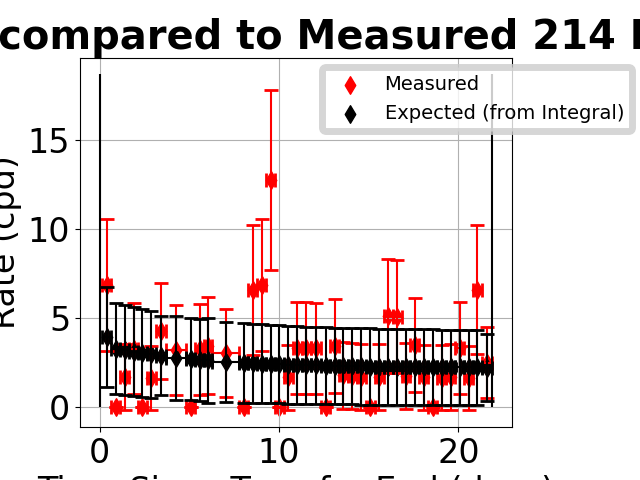
\includegraphics[scale=0.4]{Expected_compared_to_Measured_214_Run_733_C.png}
\end{figure}
\begin{figure}
	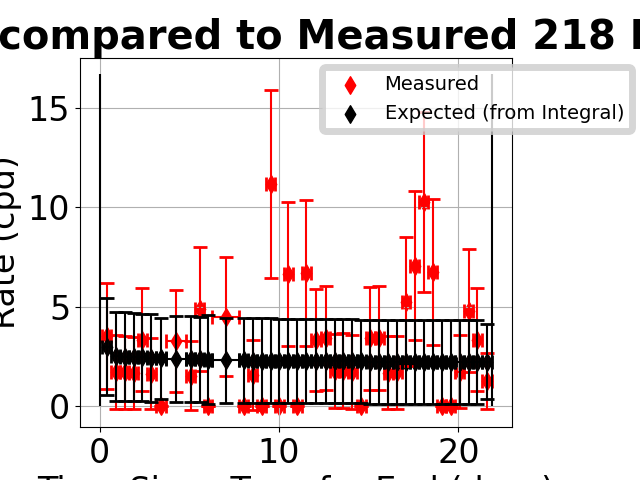
\includegraphics[scale=0.4]{Expected_compared_to_Measured_218_Run_733_C.png}
\end{figure}

\end{document}
